\documentclass[11pt,a4paper,DIVcalc,BCOR8mm,titlepage,twoside]{scrartcl}

%\usepackage[parfill]{parskip}    % Activate to begin paragraphs with an empty line rather than an indent
\usepackage{german}
\usepackage{amsmath}
\usepackage{amsfonts}
\usepackage{amssymb}
\usepackage{graphicx}
\usepackage{natbib}
\bibpunct{(}{)}{;}{a}{}{,} % to follow the A&A style

\begin{document}
	\titlehead{Christian--Albrechts--Universit"at zu Kiel\\ Institut f"ur Theoretische Physik und Astrophysik}
	\subject{Diplomarbeit}
	\title{L"osung des Strahlungstransportproblems in Pfadintegralform mit effizienten Monte--Carlo--Verfahren}
	\author{vorgelegt von Thies Heidecke\\(theidecke@astrophysik.uni-kiel.de)}
	\publishers{betreut durch Prof. Sebastian Wolf}
	\date{Version vom \today}
	\maketitle
	% standard-titelblatt verf"ugbar?

	\tableofcontents
	\vfill
	\pagebreak
	
	\newcommand{\location}[1]{\mathbf{#1}}
	\newcommand{\scatter}[1]{\overset{#1}{\leftrightsquigarrow}}
	\newcommand{\normalized}[1]{\frac{#1}{||#1||}}
	
	\section{Einleitung}
	\subsection{Motivation}
	TODO: astrophysikalischer Kontext $\rightarrow$ Begr"undung der in Sektion (\ref{sec:radiative_transfer}) gemachten Annahmen
	\subsection{Ziele der Arbeit}
	In dieser Arbeit soll eine Pfadintegraldarstellung der Strahlungstransportgleichung hergeleitet werden, sowie dessen Nutzen f"ur Monte--Carlo--Verfahren zur L"osung des Strahlungstransportproblems theoretisch und praktisch in Form eines Computerprogrammes gezeigt werden.
	
	\subsection{Nomenklatur}
	Im folgenden Text werden die in Tabelle \ref{tab:nomenklatur} angegebenen Schreibweisen benutzt.

	\begin{table}
		\caption{Nomenklatur}
		\begin{center}
		\begin{tabular}{rll}
			Schreibweise & Bedeutung & Einheit \\
			\hline
			$\kappa$ & Volumenabsorptionsquerschnitt & $\left[\text{m}^2/\text{m}^3\right]$ \\
			$\sigma$ & Volumenstreuquerschnitt & $\left[\text{m}^2/\text{m}^3\right]$ \\
			$\xi$ & Volumenextinktionsquerschnitt & $\left[\text{m}^2/\text{m}^3\right]$ \\
			$\varepsilon$ & Volumenemissivit"at & $\left[\text{W}/(\text{m}^3\,\text{sr})\right]$ \\
			$I(\location{r},\omega)$ & Intensit"at am Ort $\location{r}$ in Richtung $\omega$& $\left[\text{W}/(\text{m}^2\,\text{sr})\right]$ \\
			$W(\location{r},\omega)$ & Sensitivit"at am Ort $\location{r}$ in Richtung $-\omega$ & $\left[(\text{m}^2\,\text{sr})/\text{W}\right]$ \\
			$\phi(\location{r},\omega',\omega)$ & Phasenfunktion am Ort $\location{r}$ f"ur ein Teilchen, & $\left[1/\text{sr}\right]$ \\
				&das sich vor der Streuung in Richtung $\omega'$&\\
				&und nach der Streuung in Richtung $\omega$ bewegt& \\
			$\scatter{i}$ & Phasenfunktion am Ort $\location{r}_i$ f"ur ein aus Richtung $\location{r}_{i-1}$&\\ 
				&kommendes und in Richtung $\location{r}_{i+1}$ gestreutes Teilchen&\\
				&("aquivalent zu $\phi(\location{r}_i,\normalized{\location{r}_i-\location{r}_{i-1}},\normalized{\location{r}_{i+1}-\location{r}_i})$)& \\
			$\tau_{i,j}$ & Optische Tiefe zwischen $\location{r}_i$ und $\location{r}_j$ & \\
			$\varepsilon_{i,j}$ & Emissivit"at am Ort $\location{r}_i$ in Richtung $\location{r}_j$ & \\
			$W_{j,i}$ & Sensitivit"at am Ort $\location{r}_i$ in Richtung $-\normalized{\location{r}_j-\location{r}_i}$ &
		\end{tabular}
		\end{center}
		\label{tab:nomenklatur}
	\end{table}
	
	
	\section{Das Strahlungstransportproblem}
	\label{sec:radiative_transfer}
	
	Das Verhalten von Licht l"asst sich (nach heutigem wissenschaftlichen Stand) durch die {\em Quantenelektrodynamik} in allen Details vollst"andig beschreiben. Es beinhaltet solche Ph"anomene wie Dispersion, Brechung, Interferenz, Photon--Photon--Interaktion, etc. Diese Effekte sind h"aufig dann am bedeutendsten, wenn die Ausma"se der betrachteten Objekte von der Gr"o"senordnung der Wellenl"ange des Lichtes sind. Auf der anderen Seite beschreibt die {\em geometrische Optik} die rein makroskopische lineare Ausbreitung gro"ser Mengen von Photonen ohne obengenannte Wellen--Ph"anomene zu ber"ucksichtigen.
	
	Beim Strahlungstransportproblem (STP) sind wir an einer {\em ph"anomenologischen} Beschreibung interessiert. Das heisst wir wollen die Effekte des Lichtes modellieren, die in typischen Anwendungen durch optische Instrumente (Auge, Teleskope mit Photoplatten/CCD--Chips) gemessen werden k"onnen. Dies bedeutet, das wir haupts"achlich eine geometrische Beschreibung des Lichtes in Form eines Teilchentransportproblems ansetzen aber relevante quantenmechanische Effekte wie Photonen--Streuung in erster Ordnung lokal mitber"ucksichtigen (z.B. in Form einer Streuphasenfunktion).
	
	Die folgende Darstellung und Herleitung orientiert sich an \citep{Arvo:1993p9035}
	
	\subsection{Das Strahlungstransportproblem als Teilchentransportproblem}
	Um Strahlungstransport als Teilchentransportproblem behandeln zu k"onnen m"ussen folgende Bedingungen erf"ullt sein
	\begin{itemize}
		\item{Die Teilchen m"ussen so klein und zahlreich sein, das ihre statistische Verteilung als kontinuierlich angesehen werden kann}
		\item{Zu jedem Zeitpunkt l"asst sich ein Teilchen komplett durch seinen Positionsvektor, Geschwindigkeitsvektor und eventuelle interne Zust"ande (wie Polarisation, Frequenz, Ladung, Spin, etc.) charakterisieren}
	\end{itemize}
	Diese Annahmen sind f"ur Photonen und die uns interessierenden r"aumlichen Entfernungen erf"ullt.
	Dar"uber hinausgehend machen wir im Rahmen dieser Arbeit folgende Annahmen:
	\begin{itemize}
		\item{Die Materialeigenschaften variieren bei Variation des Ortes in der Gr"o"senordnung der Wellenl"ange nur wenig}
		\item{Das Strahlungsintensit"atsfeld ist station"ar (d.h. innerhalb der typischen Zeiten, die ein Photon braucht um das Simulationsgebiet zu durchqueren, k"onnen die Materialeigenschaften als statisch angenommen werden)}
		\item{Photonen werden ausschliesslich elastisch gestreut}
		\item{der Raum wird als euklidisch angenommen (d.h. es werden keine relativistischen Effekte ber"ucksichtigt)}
	\end{itemize}
	Die Annahme ausschliesslich elastischer Streuvorg"ange erlaubt es uns, dass Strahlungstransportproblem f"ur jede Wellenl"ange getrennt zu betrachten, da Photonen bei elastischer Streuung ihre Wellenl"ange nicht "andern und somit den Strahlungstransport in anderen Wellenl"angen nicht beeinflussen. Daher behandeln wir im Folgenden nur das monochromatische Strahlungstransportproblem, in dem Wissen, da"s der polychromatische Fall immer als eine Reihe von monochromatischen Problemen behandelt werden kann. Aufgrund der monoenergetischen Annahme ist der Teilchenimpuls und somit die Teilchengeschwindigkeit konstant. Daher reicht es zur vollst"andigen Beschreibung eines Teilchenzustandes aus, wenn wir nur die Position $\location{r}$ (entsprechend drei Freiheitsgraden) und die Bewegungsrichtung $\omega$ (entsprechend zwei Freiheitsgraden) des Teilchens angeben. Wir k"onnen nun ein Teilchen als Punkt des zugeh"origen f"unf--dimensionalen Phasenraums $\mathbb{R}^3 \times \mathcal{S}^2$ identifizieren, wobei $\mathbb{R}^3$ den euklidischen Raum und $\mathcal{S}^2$ die Einheitskugel im $\mathbb{R}^3$ meint.
	
	Um die statistische Verteilung unserer Teilchen im Phasenraum zu jedem Zeitpunkt spezifizieren zu k"onnen f"uhren wir die Phasenraumdichte $n$ ein, soda"s $$n(\location{r},\omega,t)\,d\location{r}\,d\omega$$ der Anzahl Teilchen entspricht, die sich zum Zeitpunkt $t$ in einem infinitesimalen Volumen $d\location{r}$ um $\location{r} \in \mathbb{R}^3$ befinden und sich in eine Richtung bewegen, die innerhalb eines infinitesimalen Raumwinkels $d\omega$ um $\omega \in \mathcal{S}^2$ liegt. Damit hat $n$ die Einheit $\text{m}^{-3}\text{sr}^{-1}$. Die Phasenraumdichte trifft keine Aussage "uber Materialeigenschaften oder innere Zust"ande der Teilchen, wie Masse oder Frequenz, sondern beschreibt lediglich deren Anzahldichte im Phasenraum. Physikalisch relevante Gr"osen (wie z.B. die Intensit"at) f"uhren wir sp"ater auf die Phasenraumdichte zur"uck. An dieser Stelle erlaubt die abstraktere Natur von $n$ aber eine klarere Darstellung der wesentlichen Verhaltensweisen der Teilchen. Von der Phasenraumdichte lassen sich alle f"ur uns interessanten Gr"osen prinzipiell ableiten, f"ur die folgende Herleitung ist es aber praktischer wenn wir uns die Rate der Teilchen, die eine imagin"are Fl"ache durchqueren, anschauen.
	
	Sei $d\location{A}$ eine infinitesimales Fl"achenelement, $\omega$ die Fl"achennormale von $d\location{A}$ und $d\omega$ ein infinitesimales Raumwinkelelement, das $\omega$ beinhaltet (siehe Abb.~(\ref{fig:phasespacefluxsurface})). Betrachten wir nun die Teilchen, welche die Fl"ache $d\location{A}$ in einem Zeitraum $dt$ mit Bewegungsrichtung innerhalb $d\omega$ passieren. Alle diese Teilchen liegen im Volumen $d\location{A}\,ds$ wobei $ds=v\,dt$ und $v$ die Geschwindigkeit der Teilchen ist. Nehmen wir an, da"s $\location{r}$ innerhalb diese Volumens liegt, ist die Anzahl der Teilchen $$n(\location{r},\omega,t)\,d\location{A}\,ds\,d\omega.$$ Wenn wir stattdessen aber nach der Rate fragen, mit der die Teilchen $d\location{A}$ passieren, erhalten wir den Phasenraumflu"s $$\phi(\location{r},\omega,t):=v\,n(\location{r},\omega,t)$$ mit der Einheit $[\phi]=\text{m}^{-2}\text{sr}^{-1}s^{-1}$. Die Teilchenanzahl in $d\location{A}\,ds$ mit dem Phasenraumflu"s ausgedr"uckt ist $$\phi(\location{r},\omega,t)\,d\location{A}\,d\omega\,dt.$$
	\begin{figure}
		\centering
		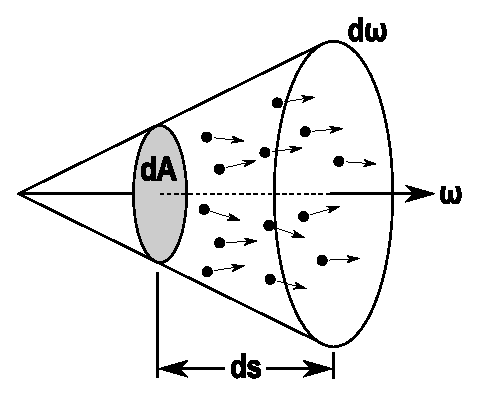
\includegraphics[height=0.3\textheight]{phasespacefluxsurface.eps}
		\caption{Teilchen, die das infinitesimale Fl"achenelement $d\location{A}$ durchqueren und sich in eine Richtung innerhalb des infinitesimalen Raumwinkelelements $d\omega$ um die Fl"achennormale $\omega$ von $d\location{A}$ bewegen.}
		\label{fig:phasespacefluxsurface}
	\end{figure}
	Der Phasenraumflu"s ist ebenso wie die Phasenraumdichte eine fundamentale Gr"ose aus der wir alle anderen interessanten Gr"osen ableiten k"onnen. Im Folgenden werden wir uns aber meist auf den Phasenraumflu"s beziehen.
		
	Unser Ziel ist es nun eine Bilanzgleichung f"ur die Teilchen in einem beliebigen Teil $V \times \Omega$ des Phasenraums (siehe Abb.~(\ref{fig:phasespacevolume})) aufzustellen. Dabei ist $V \subset \mathbb{R}^3$ ein Teilvolumen des $\mathbb{R}^3$ und $\Omega \subset \mathcal{S}^2$ ein beliebiger Raumwinkel aus der Einheitskugel $\mathcal{S}^2$. Dazu betrachten wir erst einmal die m"oglichen Gr"unde, die zu einer Ver"anderung der Teilchenzahl in unserem betrachteten Phasenraumvolumen $V \times \Omega$ f"uhren k"onnen.
	\begin{figure}
		\centering
		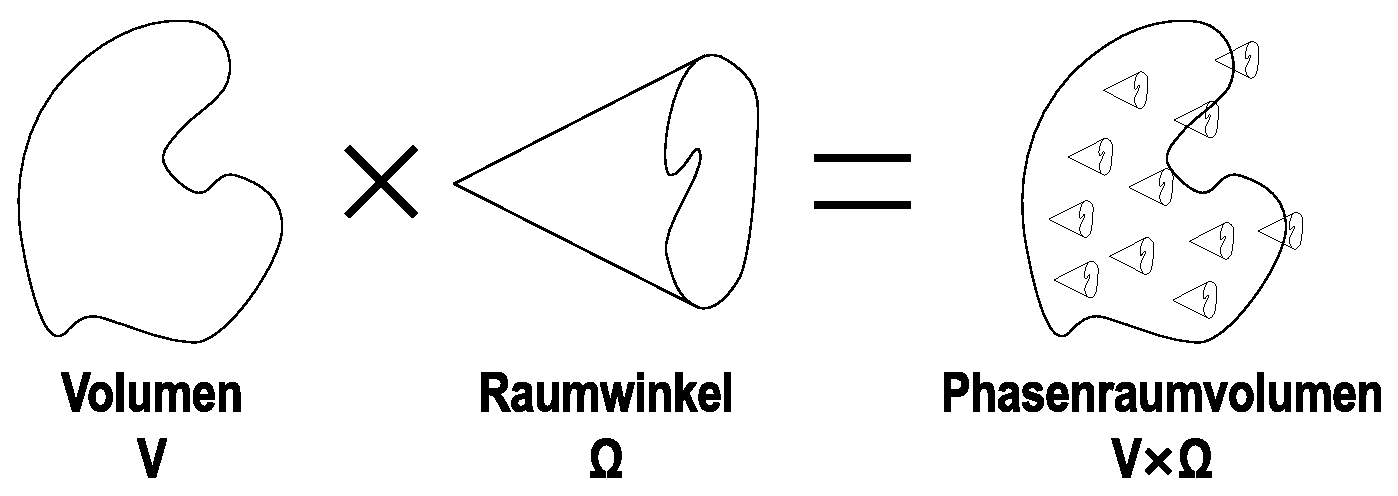
\includegraphics[width=0.8\textwidth]{phasespacevolume.eps}
		\caption{Darstellung einer Teilmenge $V \times \Omega$ des Phasenraums. Sie repr"asentiert alle Teilchen die sich innerhalb des Volumens $V$ befinden und sich in eine Richtung innerhalb von $\Omega$ bewegen.}
		\label{fig:phasespacevolume}
	\end{figure}

	Zur {\em Emission} z"ahlt jeder Prozess der neue Teilchen erzeugt. Dies kann durch verschiedene physikalische Prozesse, wie z.B. chemische Reaktionen, thermische Emission oder Kernfusion begr"undet sein. Emission innerhalb von $V$ in eine Richtung innerhalb von $\Omega$ ver"andert also die Teilchenbilanz, da sie eine Quelle f"ur Teilchen darstellt. Nach der Emission bewegen sich die Teilchen in unserem Modell gradlinig mit konstanter Geschwindigkeit bis sie eine instantane Kollision mit dem Medium erfahren. Bewegt sich ein Teilchen bei seiner gradlinigen Bewegung in das Volumen $V$ hinein oder aus ihm heraus und bewegt es sich dabei in eine Richtung innerhalb von $\Omega$, so "andert das ebenfalls unsere Teilchenbilanz. In diesem Fall sprechen wir von {\em Durchstr"omen}. Findet als letzte M"oglichkeit eine {\em Kollision} des Teilchens mit dem Medium innerhalb von $V$ statt, kann das Teilchen entweder absorbiert oder gestreut werden. Wird es absorbiert wirkt dies als Teilchensenke. Wird es gestreut, dann kann es, je nachdem in welche Richtung es sich vor und nach der Kollision bewegt hat, entweder keinen Einflu"s auf die Teilchenbilanz haben (Bewegungsrichtung vor und nach der Kollision entweder innerhalb oder ausserhalb von $\Omega$), es kann herausgestreut werden (Bewegungsrichtung vor der Kollision innerhalb und nach der Kollision ausserhalb von $\Omega$) oder aber hineingestreut werden (Bewegungsrichtung vor der Kollision ausserhalb und nach der Kollision innerhalb von $\Omega$) werden.
	
	Um die einzelnen Beitr"age dieser Prozesse zur Teilchenbilanz quantitativ zu erfassen f"uhren wir die Teilchenzahl $$N(t):=\int_\Omega \int_V n(\location{r},\omega,t)\,d\location{r}\,d\omega$$ ein. Sie gibt an wieviele Teilchen sich zum Zeitpunkt $t$ im Phasenraumvolumen $V \times \Omega$ befinden. Durch die eben beschriebenen Prozesse "andert sich $N(t)$ normalerweise mit der Zeit. Ist die Zeit, die ein Teilchen ben"otigt das betrachtete System zu durchqueren, klein gegen"uber der typischen Zeitskala, nach der sich das System bedeutend ver"andert hat, k"onnen wir annehmen, da"s sich die Teilchenzahl f"ur jedes Phasenraumvolumen im dynamischen Gleichgewicht befindet, d.h. das zwar st"andig Teilchen aus dem Phasenraumvolumen hinein- und hinausstr"omen, erzeugt, absorbiert und gestreut werden, aber sich alle Prozesse in der Bilanz die Waage halten, $N(t)$ also station"ar ist:$$\frac{dN(t)}{dt}=0\qquad\left[\frac{1}{\text{s}}\right].$$ Teilen wir diese "Anderung von $N$ mit der Zeit auf die verschiedenen obengenannten Prozessen auf sind wir bei der Grundlage einer Bilanzgleichung angelangt:$$\begin{bmatrix}\text{"Anderung}\\ \text{durch}\\ \text{Emission}\end{bmatrix}+\begin{bmatrix}\text{"Anderung}\\ \text{durch}\\ \text{Durchstr"omung}\end{bmatrix}+\begin{bmatrix}\text{"Anderung}\\ \text{durch}\\ \text{Kollisionen}\end{bmatrix}=0.$$ Wir leiten nun f"ur jeden dieser Ausdr"ucke einen Formelausdruck her.
	Die "Anderung aufgrund von Emission nennen wir $$\mathbf{E}=\int_\Omega \int_V q(\location{r},\omega)\,d\location{r}\,d\omega\qquad\left[\frac{1}{\text{s}}\right],$$ wobei wir die Phasenraumquellfunktion $q$ (mit Einheit $\text{m}^{-3}\text{sr}^{-1}\text{s}^{-1}$) eingef"uhrt haben, die f"ur jeden Ort $\location{r}$ und jede Raumrichtung $\omega$ die Anzahl erzeugter Teilchen pro Sekunde, Einheitsvolumen und Einheitsraumwinkel angibt. Hinein- und herausstr"omende Teilchen erzeugen eine Teilchenrate
	$$\mathbf{S}=\int_\Omega \int_{\partial V} \phi(\location{s},\omega)(\omega \cdot d\location{s})d\omega,$$
	die wir durch Integrieren "uber $\partial V$ (die Oberfl"ache von V) erhalten. Hierbei steht $\location{s}$ f"ur ein infinitesimales als Vektor repr"asentiertes Fl"achenelement, dessen Richtung die Fl"achennormale, und dessen L"ange seine Fl"ache repr"asentiert. Das Skalarprodukt zwischen Bewegungsrichtung $\omega$ und Fl"achennormalen sorgt f"ur das richtige Vorzeichen, wobei ein positiver Wert Teilchenverlust bedeutet.
	Der letzte Beitrag $\mathbf{C}$ tr"agt den Kollisionen Rechnung. Da Teilchen nur mit dem Medium nicht aber untereinander interagieren mu"s die Kollisionsrate unabh"angig von $\phi$ sein. Wir unterteilen $\mathbf{C}$ in einen Absorptionsteil $\mathbf{C}_\text{abs}$ und einen Streuanteil $\mathbf{C}_\text{sca}$. Wir nehmen an, da"s die Wahrscheinlichkeit, da"s ein Teilchen aufgrund von Absorption verschwindet proportional zur zur"uckgelegten Distanz im Medium, nicht aber von der Bewegungsrichtung durch das Medium ist (was gleichbedeutend mit der Annahme eines isotropen Mediums ist). Die Proportionalit"atskonstante am Ort $\location{r}$ nennen wir den (Volumen-)Absorptionsquerschnitt $\kappa(\location{r})$ ($[\kappa]=\frac{1}{\text{m}}=\frac{m^2}{m^3}$). Die zugeh"orige Teilchenrate ist
	$$\mathbf{C}_\text{abs}=\int_\Omega \int_V \kappa(\location{r})\phi(\location{r},\omega)\,d\location{r}\,d\omega.$$
	Die genauen Mechanismen der Streuung k"onnen durch Mie--Theorie oder Quantenmechanik behandelt werden. In unserem Teilchentransport repr"asentieren wir diese Streumodelle durch die Streuphasenfunktion $k(\location{r},\omega,\omega')$ und den (Volumen-)Streuquerschnitt $\sigma(\location{r})$. Dabei gibt $k(\location{r},\omega,\omega')$ bei Streuung eines aus Richtung $\omega$ kommenden Teilchens am Ort $\location{r}$ die Wahrscheinlichkeit pro Einheitsraumwinkel an, nach $\omega'$ gestreut zu werden. Da ein gestreutes Teilchen irgendwohin gestreut wird, gilt f"ur $k$ die Normierungsbedingung
	\begin{equation}\label{eq:k_norm_req}
	  \int_{\mathcal{S}^2} k(\location{r},\omega,\omega')\,d\omega'=1,
	\end{equation}
	die z.B. durch die isotrope Streuphasenfunktion $$k_\text{iso}(\location{r},\omega,\omega')=\frac{1}{4\pi}$$ erf"ullt wird. Wie bei der Absorption, nehmen wir an, da"s die Wahrscheinlichkeit eines Teilchens gestreut zu werden sehr wohl von der durch das Medium zur"uckgelegten Distanz, nicht aber von der Bewegungsrichtung abh"angt. Wir teilen $\mathbf{C}_\text{sca}$ weiter auf, in einen Teil
	$$\mathbf{C}_\text{out}=\int_\Omega \int_V \int_{\mathcal{S}^2} \sigma{(\location{r})}k(\location{r},\omega,\omega')\phi(\location{r},\omega)\,d\omega'\,d\location{r}\,d\omega,$$
	der herausgestreute Teilchen ber"ucksichtigt, sowie einen Teil
	$$\mathbf{C}_\text{in}=\int_\Omega \int_V \int_{\mathcal{S}^2} \sigma{(\location{r})}k(\location{r},\omega',\omega)\phi(\location{r},\omega')\,d\omega'\,d\location{r}\,d\omega$$
	entsprechend f"ur hineingestreute Teilchen. Dabei sollte erw"ahnt werden, da"s sowohl $\mathbf{C}_\text{out}$ als auch $\mathbf{C}_\text{in}$ Teilchen ber"ucksichtigen, deren Richtung vor und nach der Streuung in $\Omega$ liegt, was weder einem Zuwachs noch einem Verlust an Teilchen entspricht. Da f"ur unsere Bilanz aber immer nur die Differenz von $\mathbf{C}_\text{out}$ und $\mathbf{C}_\text{in}$ betrachtet wird, hebt sich dieser Teil wieder heraus. Alternativ k"onnten wir auch "uber $\mathcal{S}^2 \setminus \Omega$ integrieren, was zu einer komplizierteren Rechnung, aber zu keinem anderen Endergebnis f"uhren w"urde. F"ugen wir die Einzelterme zusammen und ordnen nach Zuw"achsen und Verlusten sieht unsere Bilanzgleichung f"ur die Teilchenraten in $V \times \Omega$ wie folgt aus:
	$$\underbrace{\mathbf{S}+\mathbf{C}_\text{abs}+\mathbf{C}_\text{out}}_\text{Verluste}=\underbrace{\mathbf{E}+\mathbf{C}_\text{in}}_\text{Zuw"achse}$$
	Es f"allt bei der Betrachtung der Formeln f"ur die einzelnen Terme auf, da"s alle Terme, bis auf $\mathbf{S}$ Volumenintegrale "uber $V \times \Omega$ enthalten. $\mathbf{S}$ enth"alt stattdessen ein Oberfl"achenintegral "uber $\partial V$. Mithilfe des Gauss'schen Satzes dr"ucken wir das Oberfl"achenintegral "uber $\partial V$ durch ein Volumenintegral "uber $V$ aus und erhalten
	$$\mathbf{S}=\int_\Omega \int_V \omega \cdot (\nabla\phi)(\location{r},\omega)\,d\location{r}\,d\omega,$$
	wobei wir $\nabla \cdot(\omega\phi)=\omega\cdot(\nabla\phi)$ benutzt haben.
	
	In unserer Bilanzgleichung treten jetzt nur noch Volumenintegrale "uber unser Phasenraumvolumen $V \times \Omega$ auf. Da $V$ und $\Omega$ beliebig gew"ahlt waren, mu"s die Bilanzgleichung "uberall und in alle Richtungen lokale G"ultigkeit haben:
	\begin{multline*}
	  \omega\cdot\nabla\phi(\location{r},\omega)+\kappa(\location{r})\phi(\location{r},\omega)+\int_{\mathcal{S}^2}\sigma(\location{r})k(\location{r},\omega,\omega')\phi(\location{r},\omega)d\omega' \\
	  =q(\location{r},\omega)+\int_{\mathcal{S}^2}\sigma(\location{r})k(\location{r},\omega',\omega)\phi(\location{r},\omega')d\omega'
	\end{multline*}
	Da beim $\mathbf{C}_\text{out}$--Integral $\sigma$ und $\phi$ nicht von der Integrationsvariable abh"angen und das verbleibende Integral aufgrund der Normierungsbedingung (\ref{eq:k_norm_req}) gleich eins ist verinfacht sich unsere Bilanzgleichung schlu"sendlich zu
	\begin{equation}\label{eq:particle_balance_equation}
	  \omega\cdot\nabla\phi(\location{r},\omega)+\left(\kappa(\location{r})+\sigma(\location{r})\right)\phi(\location{r},\omega)
	  =q(\location{r},\omega)+\sigma(\location{r})\int_{\mathcal{S}^2}k(\location{r},\omega',\omega)\phi(\location{r},\omega')d\omega'
	\end{equation}
	
	\subsection{Die Messgleichung}
	\subsection{Ph"anomenologische Strahlungsgr"o"sen}
	\subsection{Strahlungstransportgleichung in differentieller Form}
	\subsection{"Ubersicht etablierter L"osungsverfahren}
	TODO: "Ubersicht benutzter L"osungsverfahren, Meilensteine (wann zum ersten mal Polarisation gerechnet?, Warum etablieren sich MC-Verfahren so sp"at?, etc...)
		
	\section{Pfadintegralformulierung der Strahlungstransportgleichung}
	TODO: STG in diff. Form, STG in integraler From, STG in Operator--Form, Messungen als Pfadintegrale
	\subsection{Strahlungstransportgleichung in integraler Form}
	TODO: STG in integraler From
	\subsection{Strahlungstransportgleichung in Operator--Form}
	TODO: STG in Operator--Form
	\subsection{KG--Operator in Volumenform}
	\subsection{Pfadintegrall"osung der Strahlungstransportgleichung}
	TODO: Messungen als Pfadintegrale
	\subsection{Strahlungstransport als Integrationsproblem}
	
	\section{Monte--Carlo--Integration}
	\subsection{Grundlegende Begriffe aus der Statistik}
	TODO: Begriffe aus Wahrscheinlichkeitsrechnung und Statistik einf"uhren
	\subsection{Das Integrationsproblem}
	TODO: Das Integrationsproblem
	\subsubsection{Vergleich von Tensor--Produkt--Verfahren und einfacher Monte--Carlo--Integration}
	TODO: (Curse~of~Dimensionality / Konvergenzraten)
	\subsection{Importance--Sampling}

	\subsection{Monte--Carlo--Markov--Chain--Verfahren}
	\subsubsection{Metropolis--Hastings--Algorithmus}
	TODO: Metropolis--Hastings--Algorithmus
	\subsubsection{Detailed Balance}
	TODO: Detailed Balance
	\subsubsection{Generalisierter Metropolis--Hastings--Algorithmus}
	TODO: Robuste MH--Variante

	\section{Monte--Carlo--Strahlungstransport}
	\subsection{Pfadgenerierung}
	\subsubsection{Raycasting}
	\subsubsection{Distanzsampler}
	TODO: uniform depth sampler, uniform attenuation sampler, enforced uniform attenuation sampler
	
	TODO: Pfadgenerierung, Sch"atzer
	
	\section{Testf"alle und Resultate}
	\subsection{Homogene streuende Kugel}
	TODO: Motivation? tau=0.01,1,10
	\subsubsection{analytische L"osung}
	\subsubsection{Resultate}
	TODO: Vergleich mit analytischer L"osung und MC3D (Ergebnis+Geschwindigkeit)
	\subsection{Einfaches Scheibenmodell}
	\subsubsection{Resultate}
	TODO: Vergleich mit MC3D (Ergebnis und Geschwindigkeit)
	\subsection{Einordnung der Resultate}
	TODO: Gesamtvergleich zwischen MC3D und PIRaTE
	
	\section{Programmbeschreibung}
	TODO: Programmbeschreibung in Worten bzw. Pseudocode, Modulbeschreibung, Details in evtl. Anhang auslagern.
	
	\section{Zusammenfassung und Ausblick}
	TODO: Ausblick: Normierung, physikalisch relevante Streuphasenfunktionen, polychromatische Bilder/SEDs

	\bibliographystyle{chicago}
	\bibliography{bibliography}
\end{document}